\section{Actividad 11}

Transmisor FM (Fig.~\ref{fig:4}) con salida 97.9 MHz y desviación 75 kHz.  

\begin{figure}[h!]
    \centering
    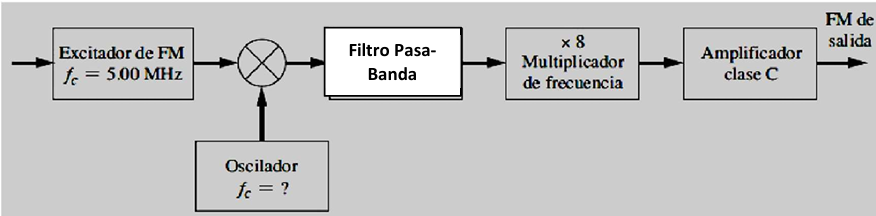
\includegraphics[width=0.6\textwidth]{fig4.png}
    \caption{Diagrama de bloques transmisor FM}
    \label{fig:4}
\end{figure}

\begin{itemize}
    \item[a)] Ancho de banda y frecuencia central del filtro.  
    \item[b)] Frecuencia del oscilador.  
    \item[c)] Capacidad de desviación pico requerida.  
    \item[d)] Índice de modulación.  
    \item[e)] Separación de frecuencias laterales adyacentes.  
\end{itemize}